%%%%%%%%%%%%%%%%%%%%%%%%%%%%%%%%%%%%%%%%%
% fphw Assignment
% LaTeX Template
% Version 1.0 (27/04/2019)
%
% This template originates from:
% https://www.LaTeXTemplates.com
%
% Authors:
% Class by Felipe Portales-Oliva (f.portales.oliva@gmail.com) with template 
% content and modifications by Vel (vel@LaTeXTemplates.com)
%
% Template (this file) License:
% CC BY-NC-SA 3.0 (http://creativecommons.org/licenses/by-nc-sa/3.0/)
%
%%%%%%%%%%%%%%%%%%%%%%%%%%%%%%%%%%%%%%%%%

%----------------------------------------------------------------------------------------
%	PACKAGES AND OTHER DOCUMENT CONFIGURATIONS
%----------------------------------------------------------------------------------------

\documentclass[
	12pt, % Default font size, values between 10pt-12pt are allowed
	%letterpaper, % Uncomment for US letter paper size
	%spanish, % Uncomment for Spanish
]{fphw}

% Template-specific packages
\usepackage[utf8]{inputenc} % Required for inputting international characters
\usepackage[T1]{fontenc} % Output font encoding for international characters
\usepackage{mathpazo} % Use the Palatino font
\usepackage{setspace}

\usepackage{graphicx} % Required for including images

\usepackage{booktabs} % Required for better horizontal rules in tables

\usepackage{listings} % Required for insertion of code

\usepackage{enumerate} % To modify the enumerate environment

\usepackage{parskip}% http://ctan.org/pkg/parskip

\usepackage{amsmath}

\usepackage{amssymb}

\usepackage{caption}

\usepackage{tikz}
\newcommand*\circled[1]{\tikz[baseline=(char.base)]{
            \node[shape=circle,draw,inner sep=2pt] (char) {#1};}}

            \usetikzlibrary{decorations.pathreplacing,positioning, arrows.meta}

            \newcommand{\ImageWidth}{\textwidth}

\usepackage{enumitem}

\usepackage[ruled,portuguese,onelanguage,longend]{algorithm2e} %for psuedo code}% http://ctan.org/pkg/algorithm2e
% \makeatletter
% \renewcommand{\@algocf@capt@plain}{above}% formerly {bottom}
% \makeatother

\usepackage{multicol}
%----------------------------------------------------------------------------------------
%	ASSIGNMENT INFORMATION
%----------------------------------------------------------------------------------------

\title{AULA 11 - Teste de Software} % Assignment title

\author{AVC, JPP, PC} % Student name

\date{} % Due date

\institute{Pontifícia Universidade Católica do Rio de Janeiro \\ Departamento de Informática} % Institute or school name

\class{Programação Modular (INF1301)} % Course or class name

\professor{Flavio Bevilacqua} % Professor or teacher in charge of the assignment

%----------------------------------------------------------------------------------------

\begin{document}

\maketitle % Output the assignment title, created automatically using the information in the custom commands above

%----------------------------------------------------------------------------------------
%	ASSIGNMENT CONTENT
%----------------------------------------------------------------------------------------
\begin{doublespace}

    \begin{enumerate}[label=\textbf{\arabic*)}]

        \item \textbf{Definição:}

              Método de controle de qualidade baseado na execução de experimentos controladoscom o objetivo de encontrar erros na aplicação.

              Devemos testar o máximo possível para que a gama de usos que o usuário fará não encontre erro. Quanto mais testamos, menor a chance do usuário encontrar um erro.

              Existem dois tipos de manutenção, corretiva e evolutiva. Manutenção Corretiva ocorre quando algo na aplicação não está de acordo com os requisitos. Manutenção evolutiva ocorre quando o cliente deseja algo que não está nos requisitos. O cliente não paga pela manutenção corretiva, mas paga pela evolutiva.

              Casos de teste começão a ser elaborados durante a documentação de requisitos.

              Antes de realizar os testes:

              \begin{itemize}
                  \item Critérios de seleção de casos de teste. Aplicações que possuem algorítmos complexos usam testes de caixa aberta.
                  \item Cenários de teste:
                        \begin{itemize}
                            \item Modo de uso do artefato.
                            \item Organização necessária.
                            \item Ferramentas.
                            \item Definição e povoamento de base.
                            \item Pessoas envolvidas no teste.
                            \item Massa de teste.
                            \item Resultados esperados.
                        \end{itemize}

              \end{itemize}

        \item \textbf{Processo de Teste de um Programa}

              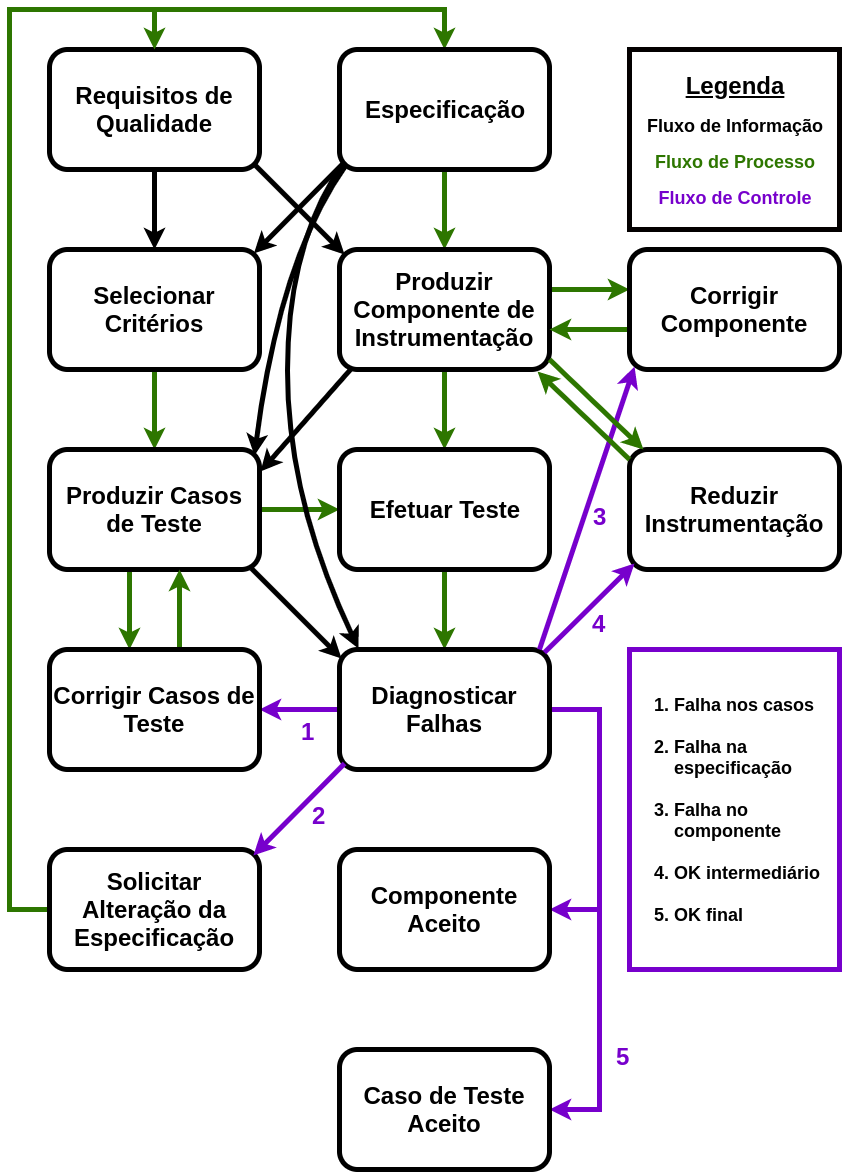
\includegraphics[width=0.9\textwidth]{2.png}

              Testagem mais rigorosa é utilizada em aplicações críticas (serviços com elevado valor ou risco grande).

              Testagem menos rigorosa é utilizada em serviços de baixo valor ou risco pequeno.

              Testes são utilizados para detectar a presença de erros, nunca a ausência de erros.

        \item \textbf{Registro de Falhas:}

              Planilha com a seguinte sugestão de campos:

              \begin{enumerate}

                  \item Data

                  \item idTeste

                  \item Sintoma

                  \item Data de correção

                  \item Artefatos alterados

                  \item Classe da falha (conjunto ao qual ela pertence, ex: especificação projeto, código, plataforma, rede, etc.)

                  \item Correção realizada

              \end{enumerate}

        \item \textbf{Critérios de Seleção de Casos de Teste:}

              Teste Caixa Fechada: são casos de teste gerados gerados a partir das especificações (input e output ou AE e AS).

              Teste Caixa Aberta: São casos de teste gerados a partir da estrutura do código. Contadores de cobertura. Deve percorrer todos os caminhos do código.

              Teste Estrutura de Dados: São casos de teste gerados a partir das assertivas estruturais e dos modelos das estruturas de dados utilizadas.

              OBS: o critério é válido quando acusa fala quando há um erro no artefato, confiável quando acusa falha independente da escolha de dados ou ações, completo quando cobre todas as condições definidas por um padrão de completeza (todos os caminhos ou todas as situações de retorno), eficaz quanto mais erros encontra e eficiente quanto menos recursos gastar.

        \item \textbf{Processo de Geração de Casos de Teste:}

              \begin{itemize}

                  \item Caso de teste abstrato (o quê?)

                        Ex: A repetição deve ocorrer três vezes.

                  \item Caso de teste semântico (como?)

                        Ex: Para que a repetição ocorra três vezes é preciso é preciso que o arquivo contenha três registros.

                  \item Caso de teste valorado ou simplesmente caso de teste

                        Ex: Inclusão dos registros de teste necessários na base e execução da aplicação a ser testada.

              \end{itemize}

        \item \textbf{Recomendações Básicas de Valoração de Casos de Teste:}

              \begin{itemize}

                  \item a $\geq$ b:

                        a > b (a = b + 1), a = b, a < b (a = b - 1)

                  \item Valores em campos de tamanho variável:

                        \begin{itemize}
                            \item vazio
                            \item tamMin
                            \item tamMax
                            \item tamMin - 1
                            \item tamMax + 1
                            \item tamMax - 1
                            \item tamMin + 1
                            \item conjunto de valores permitidos
                        \end{itemize}

                  \item Casos para estruturas criadas dinâmicamente:

                        Ex: Pesquisar em lista

                        \begin{itemize}

                            \item Lista vazia
                            \item Lista com um único elemento
                            \item Lista com três elementos

                        \end{itemize}

                        Ex: Pesquisa em árvore

                        \begin{itemize}

                            \item Árvore vazia
                            \item Árvore com um único nível
                            \item Árvore com três níveis

                        \end{itemize}

                        OBS: sempre testar utilizando os valores-limite, pois é nas extremidades que ocorre o maior número de erros.

                  \item Pesquisa num vetor com três ou mais elementos:
                        \begin{center}
                            \begin{tabular}{ | c | c | c | c | }
                                \hline
                                a & b & c & d \\
                                \hline
                            \end{tabular}
                        \end{center}


                        \begin{itemize}
                            \item Elemento no início (a)
                            \item Elemento no final (d)
                            \item Elemento no meio (b ou c)
                            \item Elemento que não está no vetor (e)
                        \end{itemize}

                  \item Teste de repetição

                        Ex: Coloca A em todos os índices do vetor

                        \begin{center}
                            \begin{tabular}{ | c | c | c | c | c | }
                                \hline
                                A & A & A & \_ & \_ \\
                                \hline
                            \end{tabular}

                            \begin{tabular}{ c c c c c }
                                I & C & C &  & \\
                            \end{tabular}
                        \end{center}

                        O terceiro A é colocado em um índice calculado sobre outro índice calculado. Arrasto = 3 - 1 = 2.

                        Ex: Fibonacci no vetor

                        \begin{center}
                            \begin{tabular}{ | c | c | c | c | c | c | }
                                \hline
                                1 & 1 & 2 & 3 & 5 & \_ \\
                                \hline
                            \end{tabular}

                            \begin{tabular}{ c c c c c c c }
                                I & I & C & C & C &  & \\
                            \end{tabular}
                        \end{center}

                        O quinto valor é calculado sobre outros dois valores calculados calculado. Arrasto = 5 - 1 = 4.

                        Arrasto é o menor número de repetições necessárias para que a próxima iteração dependa única e exclusivamente de valores calculados em repetições anteriores.

              \end{itemize}

        \item \textbf{Padrões de Cobertura de Testes Caixa Aberta}

              \begin{center}
                  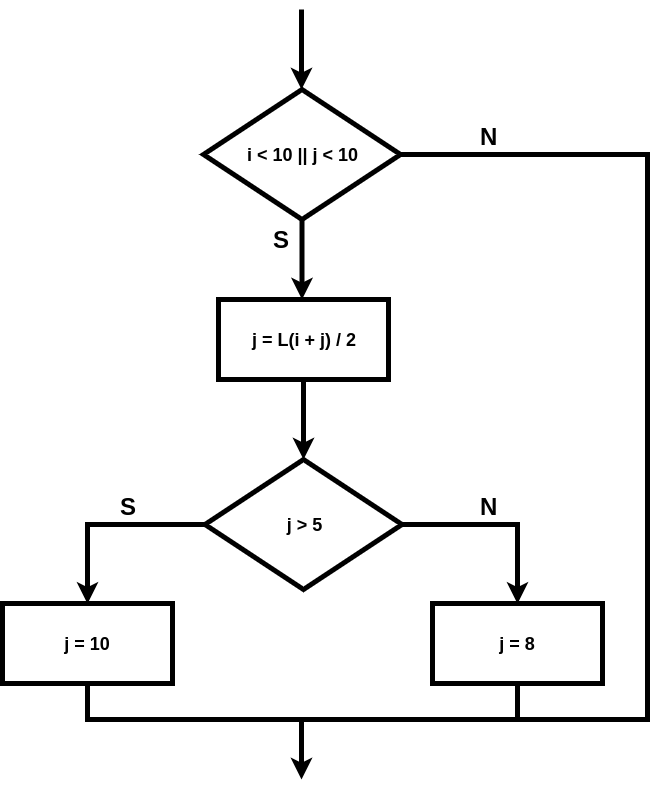
\includegraphics[width=0.75\textwidth]{DiagramaCaixaAberta.png}
              \end{center}

              \begin{center}

                  \bigskip
                  \bigskip

                  Cobertura de Decisões

                  \begin{multicols}{2}

                      \begin{enumerate}[label=\protect\circled{\arabic*}]

                          \item
                                \begin{tabular}{ | c | c | }
                                    \hline
                                    i < 10 & j < 10 \\
                                    \hline
                                    S      & S      \\
                                    S      & N      \\
                                    N      & S      \\
                                    N      & N      \\
                                    \hline
                                \end{tabular}

                                \columnbreak
                          \item
                                \begin{tabular}{ | c | }
                                    \hline
                                    j > 5 \\
                                    \hline
                                    S     \\
                                    N     \\
                                    \hline
                                \end{tabular}

                      \end{enumerate}

                  \end{multicols}


                  \begin{tabular}{ | c | c c c c c c c c | }
                      \hline
                      Caso        & 1   & 2   & 3   & 4   & 5   & 6   & 7         & 8         \\
                      i           & 4   & 1   & 2   & 1   & 10  & 10  & 10        & 10        \\
                      j           & 4   & 9   & 10  & 10  & 2   & 1   & 10        & 10        \\
                      \circled{1} & S S & S S & S N & S N & N S & N S & N N       & N N       \\
                      \circled{2} & S   & N   & S   & N   & S   & N   & Não Testa & Não Testa \\
                      \hline
                  \end{tabular}

                  \bigskip
                  \bigskip

                  Cobertura de Arestas

                  \begin{multicols}{2}

                      \begin{enumerate}[label=\protect\circled{\arabic*}]

                          \item
                                \begin{tabular}{ | c | }
                                    \hline
                                    i < 10 || j < 10 \\
                                    \hline
                                    S                \\
                                    N                \\
                                    \hline
                                \end{tabular}

                                \columnbreak

                          \item
                                \begin{tabular}{ | c | }
                                    \hline
                                    j > 5 \\
                                    \hline
                                    S     \\
                                    N     \\
                                    \hline
                                \end{tabular}

                      \end{enumerate}

                  \end{multicols}

                  \begin{tabular}{ | c | c c c c | }
                      \hline
                      Caso        & 1 & 2  & 3         & 4         \\
                      i           & 4 & 1  & 10        & 10        \\
                      j           & 9 & 10 & 10        & 10        \\
                      \circled{1} & S & S  & N         & N         \\
                      \circled{2} & S & N  & Não Testa & Não Testa \\
                      \hline
                  \end{tabular}

                  \bigskip
                  \bigskip

                  Cobertura de Comandos

                  \begin{multicols}{2}

                      \begin{enumerate}[label=\protect\circled{\arabic*}]

                          \item
                                \begin{tabular}{ | c | }
                                    \hline
                                    i < 10 || j < 10 \\
                                    \hline
                                    S                \\
                                    \hline
                                \end{tabular}

                                \columnbreak

                          \item
                                \begin{tabular}{ | c | }
                                    \hline
                                    j > 5 \\
                                    \hline
                                    S     \\
                                    N     \\
                                    \hline
                                \end{tabular}

                      \end{enumerate}

                  \end{multicols}

                  \begin{tabular}{ | c | c c | }
                      \hline
                      Caso        & 1 & 2  \\
                      i           & 4 & 1  \\
                      j           & 9 & 10 \\
                      \circled{1} & S & S  \\
                      \circled{2} & S & N  \\
                      \hline
                  \end{tabular}

              \end{center}

        \item \textbf{Teste de Caixa Fechada}

              Casos de teste gerados a partir da especificação. O teste é completo quando todas as condições de retorno são testadas. O método principal é o de partição em classes de equivalência, que são conjuntos de casos de teste que possuem o mesmo objetivo. O teste é eficiente quando gasta menos recursos. O objetivo é gerar um teste para cada classe de equivalência.

              Passo 1: Gerar os grupos principais de teste relacionados com a estrutura utilizada e resultados esperados.

              Ex: Pesquisar um valor em uma estrutura sequencial (lista, vetor, etc).

              Grupos de teste em estrutura:

              \begin{itemize}
                  \item Lista vazia
                  \item Lista com um único elemento
                  \item Lista com três elementos
              \end{itemize}

              Resultados esperados:
              \begin{itemize}
                  \item Achou
                  \item Não achou
              \end{itemize}

              \pagebreak

              Passo 2: Gerar a tabela de casos de teste.

              \begin{center}
                  \begin{tabular}{ c c c c c }
                      Caso & Lista & Elemento Pesquisado & Achou & Não Achou \\
                      \hline
                      \hline
                      1    & Vazia & A                   & 0     & 1         \\
                      2    & A     & A                   & 1     & 0         \\
                      3    & A     & B                   & 0     & 1         \\
                      4    & ABC   & A                   & 1     & 0         \\
                      5    & ABC   & C                   & 1     & 0         \\
                      6    & ABC   & B                   & 1     & 0         \\
                      7    & ABC   & D                   & 0     & 1         \\
                  \end{tabular}
              \end{center}

              Passo 3: Gerar script

              ==caso1

              =crialista	0

              =pesquisa		A 1

              ==caso2

              =insere		A 0

              =pesquisa		A 0

              ==caso3

              =pesquisa		B 1

              ==caso4

              =insere		B 0

              =insere		C 0

              =pesquisa		A 0

              ==caso5

              =pesquisa		C 0

              ==caso6

              =pesquisa		B 0

              ==caso7

              =pesquisa		D 1

        \item \textbf{Testes Estatísticos:}
        
        São casos de testes gerados automaticamente, utilizando dados aleatórios. Necessita de uma aplicação, função ou módulo gerador.

        Vantagem: total automatização.

        Desvantagem: geração de casos de teste repetidos.


    \end{enumerate}


\end{doublespace}
%----------------------------------------------------------------------------------------

\end{document}
